\chapter{Gestión de la Calidad}\label{ch:gestionDeLaCalidad}

Este capítulo se enfoca en los objetivos de calidad que el equipo ha establecido para el proyecto, categorizándolos en 
objetivos de proceso y de producto, con el fin de garantizar que tanto el desarrollo del sistema como el resultado final 
cumplan con los estándares necesarios para optimizar las operaciones de búsqueda y rescate.

\section{Objetivos de Calidad}\label{sec:ojetivosDeCalidad}

Los objetivos de calidad están orientados a asegurar que el proyecto no solo se desarrolle de manera efectiva, 
sino que también entregue un producto final que cumpla con las expectativas de los usuarios y las exigencias del 
entorno operacional del MRCC.

\subsection{Objetivos de Proceso}

Estos objetivos buscan mejorar la eficiencia y eficacia en los métodos y procedimientos aplicados durante el desarrollo del proyecto:

\textbf{Adherencia a los plazos.} Es crucial que todas las actividades planificadas para cada fase del proyecto se completen dentro 
del cronograma acordado, incluyendo las entregas iterativas a los interesados clave.

\textbf{Optimización de la velocidad de desarrollo.} Se ha establecido una velocidad esperada de desarrollo de entre 15 y 20 puntos de historia por sprint,
lo que permite una planificación precisa y un flujo constante de trabajo. Esto es vital para asegurar que los entregables se entreguen a tiempo y con la calidad requerida.


\textbf{Reducción del retrabajo.} Mediante la implementación de pruebas unitarias y revisiones de casos de uso, el equipo tiene como objetivo 
limitar el retrabajo a un máximo del 10\% del total de horas trabajadas. Esto se aplica a la corrección de errores y a los cambios solicitados 
por los clientes, asegurando un uso eficiente del tiempo y los recursos.


\subsection{Objetivos de Producto}

Los objetivos del producto se centran en garantizar que el sistema final cumpla con las expectativas de los usuarios del MRCC y esté alineado 
con los estándares de la industria:

\textbf{Aprobación de usuarios.} Se espera obtener una alta satisfacción de los usuarios del MRCC y de los responsables de las operaciones SAR 
en cada fase del proyecto. Se utilizarán encuestas de satisfacción para medir esta aprobación, con una meta de obtener una puntuación entre 4.5 
y 5 en una escala de 5.

\textbf{Resolución de errores.} Un objetivo clave es corregir el 100\% de los errores identificados durante las pruebas beta antes del despliegue
final del sistema. Se dedicará el último sprint y la última versión a la corrección de estos errores, asegurando que el sistema sea robusto y confiable.

\textbf{Conformidad con estándares y mejores prácticas.} El sistema deberá cumplir con los estándares establecidos por la Armada Nacional y con 
las mejores prácticas internacionales en la gestión de incidentes SAR, como las estipuladas en el Manual Internacional IAMSAR. Además, se debe 
garantizar que el sistema sea fácilmente mantenible y escalable para futuras actualizaciones.
\section{Plan de Calidad}\label{sec:planDeCalidad}

Para gestionar la calidad, se elaboró un plan de calidad acorde a las fases y características del proyecto. 
La principal ventaja de vincular las fases de esta metodología con las actividades del plan de calidad es que 
estas mismas definen las entradas y salidas necesarias. Por ejemplo, para avanzar hacia la fase de Definición del 
Design Sprint, es fundamental tener un entendimiento claro del problema y una solución inicial, lo cual se logra a 
través de reuniones con el cliente, sesiones de brainstorming y encuestas, entre otras.

[cita: https://docs.google.com/document/d/1DPE-N0FGD98RzhQ7z3znxXckbE4x95Swp8Z4S-LJYh0/edit?usp=sharing]


\section{Aseguramiento de la Calidad}\label{sec:aseguramientoDeLaCalidad}

Para cumplir con los objetivos establecidos, se desarrolló un conjunto de prácticas que aseguran la calidad tanto en la 
gestión del proceso como en el producto final. Estas prácticas fueron adoptadas por todo el equipo y se aplicaron 
consistentemente a lo largo de todas las fases del proyecto.

\subsection{Aplicación de estándares}
Desde el inicio, se definieron estándares claros tanto para los procesos como para el producto final. Algunos de estos 
estándares fueron definidos internamente por el equipo, mientras que otros se basaron en recomendaciones de la industria.

\subsection{Estándares de codificación}
Se implementaron principios de Clean Code para garantizar una estructura y sintaxis claras en el código fuente, facilitando 
la comprensión y modificabilidad del software. El código se escribió en inglés para mejorar su legibilidad y facilitar la 
expansión futura del equipo de desarrollo. Se aplicaron los principios SOLID para asegurar que el código sea modular, fácil 
de mantener y modificado, maximizando su efectividad y reduciendo costos de mantenimiento.
En la tabla siguiente se detallan los diferentes estándares aplicados al código fuente en este proyecto.

\begin{table}[H]
    \centering
    \begin{tabular}{p{3cm} p{10cm}}
    \hline
    \rowcolor[HTML]{C0C0C0} 
    \textbf{Estándar} & \textbf{Descripción}                                                                                     \\ \hline
    \textbf{Clean Code} & Se aplicaron principios de Clean Code para garantizar una estructura y sintaxis claras en el código fuente. \\ \hline
    \textbf{SOLID}     & Se aplicaron los principios SOLID para asegurar que el código sea modular, fácil de mantener y modificar.       \\ \hline
    \textbf{Inglés}    & El código se escribió en inglés para mejorar su legibilidad y facilitar la expansión futura del equipo de desarrollo. \\ \hline
    \end{tabular}
    \caption{Estándares de codificación}
    \label{tab:estandaresCodificacion}
\end{table}

\subsection{Estándares de documentación}

Para los documentos generados durante el proyecto, se siguieron las directrices de la Universidad ORT Uruguay, 
complementadas con lineamientos específicos del equipo para garantizar coherencia y uniformidad.
En la tabla \ref{tab:estandaresDocumentacion} se detallan los diferentes estándares aplicados a la documentación en este proyecto.


\begin{table}[H]
    \centering
    \begin{tabular}{p{3cm} p{10cm}}
    \hline
    \rowcolor[HTML]{C0C0C0} 
    \textbf{Estándar} & \textbf{Descripción}                                                                                     \\ \hline
    \textbf{Normas de la Universidad ORT} & Se siguieron las directrices de la Universidad ORT Uruguay para la redacción de documentos. \\ \hline
    \textbf{Uniformidad}     & Se establecieron lineamientos específicos del equipo para garantizar coherencia y uniformidad en la documentación.       \\ \hline
    \end{tabular}
    \caption{Estándares de documentación}
    \label{tab:estandaresDocumentacion}
\end{table}

\subsection{Plan de Pruebas}
\subsubsubsection{Objetivo}

Evaluar las funcionalidades del producto de software para verificar y validar que satisface las necesidades y expectativas del cliente. El plan 
busca garantizar la calidad mediante pruebas que cubren tanto aspectos funcionales como no funcionales, con un enfoque ágil e iterativo.

\subsubsubsection{Alcance}
El plan de pruebas cubre la verificación de las funcionalidades del sistema, su compatibilidad con el ambiente de uso y la evaluación de la 
experiencia de usuario bajo condiciones realistas. Además, se incluyen pruebas de rendimiento bajo alta demanda. No se realizarán pruebas 
específicas de seguridad debido a que se asume que el sistema será utilizado en un entorno controlado y seguro.

\subsubsubsection{Equipo}
Se asginan los roles y tareas a cada integrante descritos en la tabla \ref{tab:rolesPruebas}.

\begin{table}[H]
    \centering
    \begin{tabular}{p{3cm} p{3cm} p{8cm}}
    \hline
    \rowcolor[HTML]{C0C0C0} 
    \textbf{Nombre} & \textbf{Rol} & \textbf{Responsabilidad}                                                                                     \\ \hline
    Horacio Ábalos & QA y Tester & Planificación y ejecución de pruebas funcionales y no funcionales. Cobertura de requisitos. Gestión de herramientas de automatización. Identificación y seguimiento de defectos. Colaboración en la resolución de problemas. Pruebas exploratorias. \\ \hline
    Cristian Palma & PO y Tester & Definición de la visión del producto. Priorización de backlog. Alineación de requisitos. Revisión y aceptación de entregas. Retroalimentación continua. Identificación y seguimiento de defectos. Pruebas funcionales y exploratorias. \\ \hline
    Federico Alonso & Arquitecto y Revisor de Código & Diseño y validación de la arquitectura. Decisiones sobre tecnología. Definición de componentes y su interacción. Resolución de problemas técnicos. Revisión de código y decisiones de diseño. \\ \hline
    Ramiro Gallego & Tester y Revisor de Código & Pruebas funcionales y exploratorias. Revisión y mejora de calidad de código. Identificación de defectos. Validación de la implementación y documentación de pruebas. \\ \hline
    \end{tabular}
    \caption{Roles en el equipo de pruebas}
    \label{tab:rolesPruebas}
\end{table}


\subsubsubsection{Estrategia}

\subsubsubsubsection{Risk-Based Testing}
Se implementará una matriz de riesgo para priorizar las pruebas en base a dos factores:

\begin{itemize}
    \item \textbf{Probabilidad de fallo:} complejidad de la solución, dependencia de sistemas externos.
    \item \textbf{Impacto en el negocio:} funcionalidades críticas como la gestión de incidentes, cálculo y 
    obtención de datos de barcos y meteorológicos.
\end{itemize}

% insertar una imagen
\begin{figure}[H]
    \centering
    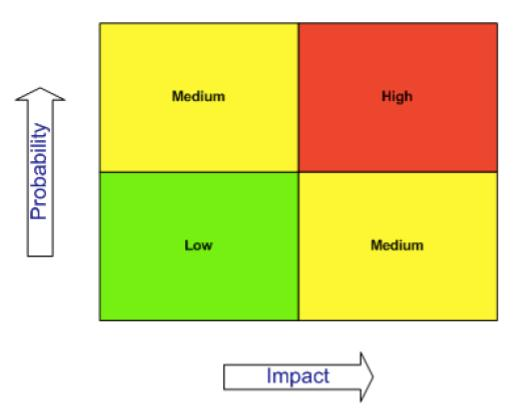
\includegraphics[width=0.8\textwidth]{../imagenes/secciones/8-Gestion-de-la-Calidad/matriz de testing basado en riesgo.jpg}
    \caption{Matriz de testing basado en riesgo}
    \label{fig:matriTestRiesgo}
\end{figure}

Esta matriz ayudará a centrar los esfuerzos de prueba en las áreas del sistema con mayor riesgo y probabilidad de impacto. 
De ella se desprende que:

\begin{itemize}
    \item Alta probabilidad y alto impacto (rojo): Debe probarse primero.
    \item Alta probabilidad y bajo impacto (amarillo): Se debe probar si hay tiempo disponible.
    \item Baja probabilidad y alto impacto (amarillo): Debe probarse si se dispone de tiempo suficiente.
    \item Baja probabilidad y bajo impacto: Se puede posponer para futuras iteraciones.
\end{itemize}

\begin{figure}[H]
    \centering
    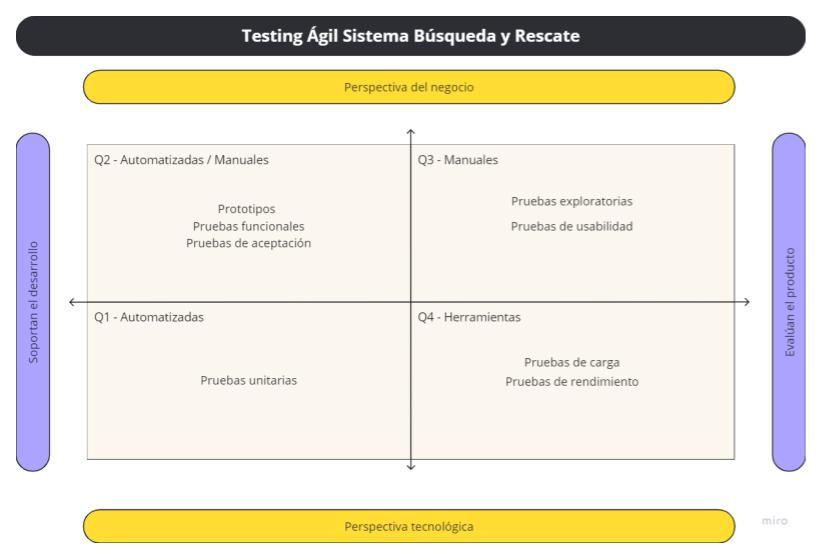
\includegraphics[width=0.8\textwidth]{../imagenes/secciones/8-Gestion-de-la-Calidad/Cuadrantes testing agil .jpg}
    \caption{Cuadrantes de testing ágil}
    \label{fig:cuadrantesTesting}
\end{figure}


\subsubsubsubsubsection{Q1 - Pruebas unitarias}
Estas pruebas serán realizadas sobre la lógica de la funcionalidad clave, el Cálculo del Área de Búsqueda, utilizando 
el framework Jest. El objetivo es asegurar que cada unidad de código funcione correctamente y de manera aislada. 
Las pruebas se ejecutarán automáticamente en cada merge a la rama develop, verificando así la estabilidad continua del sistema. 
Además, se incluirán pruebas en otras áreas de la lógica que estén acopladas a estas funcionalidades críticas para evitar regresiones.

\subsubsubsubsubsection{Q2 -  Pruebas Funcionales y de Aceptación}
\subsubsubsubsubsubsection{Pruebas funcionales}
En estas pruebas se consideran aspectos relevantes como las integraciones del sistema con servicios externos para la obtención de datos 
climáticos y la información de barcos cercanos a un incidente. Estas pruebas serán automatizadas para ejecutarse continuamente durante 
regresiones y en el pipeline de CI/CD. Se emplearán herramientas como Jest y los resultados se verificarán automáticamente en cada merge 
a la rama develop.

\subsubsubsubsubsubsection{Pruebas de aceptación}
Estas pruebas serán automatizadas utilizando Cucumber y se basarán en escenarios escritos en el formato Como [rol] quiero [funcionalidad] 
para [beneficio]. El objetivo del equipo es integrar estas pruebas en el pipeline solamente para las funcionalidades clave, permitiendo 
una rápida verificación del estado del sistema con cada merge a develop. Estas pruebas se enfocan en validar que el sistema cumple con los 
criterios de aceptación definidos por el Product Owner y las necesidades del usuario final.

\subsubsubsubsubsection{Q3 - Pruebas Exploratorias y de Usabilidad}
\subsubsubsubsubsubsection{Pruebas exploratorias}
Serán realizadas también pruebas exploratorias por diferentes integrantes del equipo. Estas pruebas deben ser ejecutadas por un integrante 
diferente al que haya desarrollado la funcionalidad.
Se utilizará la siguiente plantilla para estas sesiones exploratorias.

[link a la plantilla: https://docs.google.com/document/d/1nvdvL7GpPiP9tGPadTUYDdJpAkJrE9nZXniJSIlVs88/edit]

\subsubsubsubsubsubsection{Pruebas de usabilidad}
Considerando el contexto específico del sistema, y que será utilizado por usuarios altamente capacitados, el centro del esfuerzo no estará 
en realizar pruebas de usabilidad. Independientemente de lo anterior, realizaremos encuestas a los usuarios luego de la gestión de un incidente 
que nos proporcione la retroalimentación para verificar si el sistema es fácilmente utilizable y permite completar tareas mejorando los tiempos 
empleados actualmente.\\
En tal sentido se liberará la primera versión del sistema para validar las funcionalidades en entornos controlados y con usuarios reales. Durante 
esta primera versión se recolectará feedback utilizando encuestas post-gestión de incidente.\\
Las encuestas serán cortas y específicas, asegurándonos de recolectar retroalimentación sin interrumpir las tareas. Se implementará un sistema de 
retroalimentación multivaluado que nos permita entender si:

\begin{itemize}
    \item ¿El usuario considera necesario modificar el sistema?
    \item ¿El sistema cumple tus expectativas en cuanto a facilidad de uso?
    \item ¿Cómo es calificada la experiencia general utilizando el sistema?
    \item ¿El tiempo empleado en realizar los cálculos acorta significativamente el tiempo de las tareas?
\end{itemize}

En la siguiente plantilla se propone la encuesta inicial a ser incluida en un formulario que será visualizado luego de cerrar un incidente.

[link a la plantilla: https://docs.google.com/document/d/1uuIf-cvXXNpDl3GCFkLb5_kfsGJymRFhI9w9hSoFSag/edit]

\subsubsubsubsubsection{Q4 - Pruebas de Performance}

Las pruebas de rendimiento se realizarán utilizando K6, una herramienta especializada para simular condiciones de alta carga y estrés. El objetivo 
es evaluar cómo el sistema maneja situaciones críticas, midiendo el tiempo de respuesta, la capacidad de procesar múltiples solicitudes simultáneas y 
la estabilidad bajo picos de uso. Estas pruebas se integrarán en el pipeline de CI/CD, permitiendo detectar problemas de rendimiento en etapas tempranas 
del desarrollo. El uso de K6 permitirá automatizar las simulaciones y obtener métricas detalladas para ajustar y optimizar el rendimiento de la aplicación.

[TODO: Ajustar según los RNF finales]

\subsubsubsubsection{Criterios de Ejecución y Finalización}

\begin{itemize}
    \item Inicio: Las pruebas comenzarán una vez superadas todas las pruebas unitarias.
    \item Finalización: Las pruebas finalizarán cuando:
    \begin{itemize}
        \item Todos los casos de prueba de prioridad alta (1) se ejecuten sin fallos.
        \item Al menos el 60\% de los casos de prueba de prioridad media (2) se ejecuten sin fallos.
    \end{itemize}
\end{itemize}

La tabla \ref{prioridadCasosPrueba} establece la prioridad para la ejecución de los casos de prueba:

\begin{table}[H]
    \centering
    \begin{tabular}{p{3cm} p{10cm}}
    \hline
    \rowcolor[HTML]{C0C0C0} 
    \textbf{Prioridad} & \textbf{Descripción}                                                                                     \\ \hline
    \textbf{1} & Caso de prueba debe ser ejecutado \\ \hline
    \textbf{2} & Caso de prueba debería ser ejecutado         \\ \hline
    \textbf{3} & Caso de prueba puede ser ejecutado \\ \hline
    \end{tabular}
    \caption{Prioridad y significado de los casos de prueba}
    \label{tab:prioridadCasosPrueba}
\end{table}

\subsubsubsubsection{Ambientes}
\subsubsubsubsubsection{Pre-Producción}
Se utilizará un ambiente de pre-producción para realizar pruebas de integración y aceptación del sistema. Este ambiente tendrá las siguientes
especificaciones:

\begin{itemize}
    \item Marca: No especificado
    \item Disco: 100 GB
    \item Memoria: No especificada
    \item SO: Rocky Linux 9.4
    \item Navegador: Google Chrome v127.0.6533.100 (64 bits)
\end{itemize}

Los servicios del sistema en este ambiente estarán contenedorizados, utilizando contenedores gestionados por Podman. Esto asegura que el 
entorno de pre-producción se mantenga consistente y escalable, con la capacidad de desplegar y gestionar los servicios de manera eficiente.

\subsubsubsubsubsection{Desarrollo y Test}

\begin{itemize}
    \item Marca: Dell Inspiron
    \item SO: Linux Server 22.04
    \item Disco: 250 GB
    \item Memoria: 6 GB
    \item Navegador: Google Chrome v127.0.6533.100 (64 bits)
    \item Datos: Datos reales de buques y datos simulados para incidentes basados en ejercicios de entrenamiento realizados en cursos internacionales.
\end{itemize}

En este entorno se utilizará Docker para ejecutar los sistemas dentro de contenedores, asegurando una portabilidad total entre los ambientes de desarrollo 
y pre-producción. Las imágenes dockerizadas contendrán las aplicaciones y bases de datos necesarias para las pruebas.

\subsubsubsubsection{Entregables}

Los entregables generados en cada uno de los releases serán:

\begin{itemize}
    \item Plan de pruebas
    \item Lista de los escenarios de pruebas ejecutadas
    \item Informe de estado al finalizar cada release
    \item Reporte de defectos
\end{itemize}
\section{Gestión de Incidentes}\label{sec:gestionDeIncidentes}

El objetivo de la gestión de incidentes es identificar y registrar de manera temprana los defectos y mejoras en el producto, 
con el fin de corregirlos oportunamente. Para ello, el equipo decidió utilizar Azure DevOps para reportar los incidentes. Se detalló una 
descripción de cada incidente, las causas conocidas, el tipo (defecto o mejora), quién lo reportó, la fecha y el lugar donde fue detectado.

Los incidentes serán registrados en Azure Boards, donde se registrarán, priorizarán y gestionarán todos los problemas detectados 
durante las fases de prueba. El flujo de trabajo para cada incidente será el siguiente:

\begin{enumerate}
    \item \textbf{Registro del Incidente}\\
    El tester será responsable de registrar el incidente en Azure Boards, proporcionando una descripción detallada que incluya:
    \begin{itemize}
        \item Título breve y conciso.
        \item Severidad asignada.
        \item Pasos para reproducir el problema.
        \item Datos específicos utilizados para la prueba (si corresponde).
        \item Capturas de pantalla, registros o cualquier otro dato relevante que facilite la resolución.
    \end{itemize}
    \item \textbf{Asignación de Prioridad}\\
    El Product Owner (PO) revisará cada incidente registrado y asignará una prioridad basada en el impacto que tiene en el sistema y en los objetivos del sprint. 
    Esto asegura que los problemas más críticos se aborden primero.
    \item \textbf{Análisis y Diagnóstico}\\
    El equipo de desarrollo, junto con los revisores de código, analizará los incidentes para identificar la causa del incidente. Durante esta etapa, se puede convocar 
    a sesiones de revisión conjunta para comprender mejor el problema, discutir posibles soluciones y estimar el tiempo de corrección.
    \item \textbf{Implementación de la Solución}\\
    Una vez identificado el problema, el desarrollador asignado trabajará en la corrección. Se asegurará de:
    \begin{itemize}
        \item Realizar los cambios necesarios en el código.
        \item Ejecutar pruebas unitarias y funcionales para verificar que la solución resuelve el problema sin introducir nuevos defectos.
        \item Notificar al equipo de QA cuando la corrección esté lista para ser validada.
    \end{itemize}
    \item \textbf{Validación y Cierre}\\
    El equipo de QA ejecutará pruebas de validación para asegurar que el incidente ha sido resuelto y que no afecta otras funcionalidades. Si la solución es efectiva,
    el incidente se marcará como resuelto y se cerrará. Si persisten problemas, se reabre el incidente para un análisis adicional.
    \item \textbf{Reporte de Progreso y Estado}\\
    Periódicamente, se generarán un informe de seguimiento utilizando la siguiente plantilla que resumirá:
    \begin{itemize}
        \item Número total de incidentes reportados.
        \item Número de incidentes abiertos, en proceso y cerrados.
        \item Severidad de los incidentes pendientes.
        \item Estos informes permitirán al equipo tener una visión clara del estado del sistema y del progreso en la resolución de problemas, ayudando a tomar decisiones 
        informadas sobre la planificación de futuras iteraciones.
    \end{itemize}
    \item \textbf{Reuniones de Seguimiento}\\
    Durante las reuniones de seguimiento de sprint (retrospectivas), se revisará el estado de los incidentes y se discutirán bloqueadores o problemas recurrentes que
    necesiten atención especial. Este espacio también servirá para ajustar prioridades si se identifican nuevos riesgos o problemas críticos.
    \item \textbf{Gestión de Incidentes Recurrentes}\\
    En caso de que un mismo tipo de problema reaparezca en múltiples ocasiones, se convocará a una sesión de análisis profundo para entender las causas subyacentes.
    Para esta etapa el equipo dispone de las herramientas Pareto Ponderado y 5 Por qués.
\end{enumerate}


La gestión de los incidentes se representa a través del flujo indicado en la figura \ref{fig:flujoIncidentes}.

\begin{figure}[H]
    \centering
    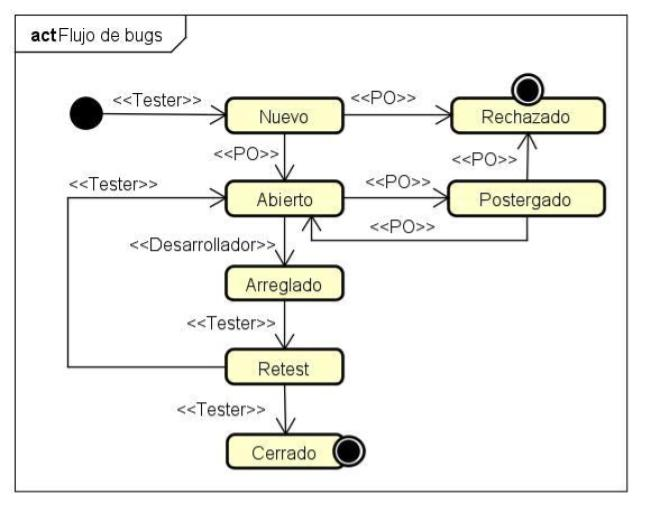
\includegraphics[width=0.8\textwidth]{../imagenes/secciones/8-Gestion-de-la-Calidad/Flujo gestion de incidentes.jpg}
    \caption{Flujo de Gestión de Incidentes}
    \label{fig:flujoIncidentes}
\end{figure}

La tabla \ref{tab:estadosIncidentes} describe los posibles estados de un incidente y su significado.

\begin{table}[H]
    \centering
    \begin{tabular}{p{3cm} p{10cm}}
    \hline
    \textbf{Estado} & \textbf{Descripción} \\ \hline
    Nuevo & El incidente ha sido registrado en Azure Boards y está pendiente de revisión por el Product Owner. \\ \hline
    Rechazado & El Product Owner ha revisado el incidente y ha determinado que no es válido o no es necesario corregirlo. \\ \hline
    Postergado & El incidente ha sido validado pero no se ha asignado a un sprint específico. \\ \hline
    Abierto & El incidente ha sido validado y asignado a un sprint específico para su corrección. \\ \hline
    Arreglado & El desarrollador ha implementado una solución y está pendiente de validación por el equipo de QA. \\ \hline
    Restest & El incidente ha sido validado por el equipo de QA y se ha detectado que la solución no es efectiva. \\ \hline
    Cerrado & El incidente ha sido validado por el equipo de QA y se ha confirmado que la solución es efectiva. \\ \hline
    \end{tabular}
    \caption{Estados de un Incidente}
    \label{tab:estadosIncidentes}
\end{table}

\subsection{Severidad de un incidente}
La severidad se clasifica en 5 niveles descritos en la tabla \ref{tab:severidadIncidentes}.

\begin{table}[H]
    \centering
    \begin{tabular}{p{3cm}p{10cm}}
    \hline
    \textbf{Severidad} & \textbf{Significado} \\ \hline
    Bloqueante & Implica que una funcionalidad no se pueda utilizar y no exista otra forma de realizar esa misma acción. El sistema falla por completo o una funcionalidad esencial no está disponible. \\ \hline
    Crítica & Implica que una funcionalidad no se puede utilizar pero existe una alternativa para completar la acción. \\ \hline
    Alta & Defecto en una funcionalidad prioritaria del sistema o que tiene impacto secundario en una funcionalidad prioritaria del mismo. Una funcionalidad importante está afectada, pero el sistema aún es utilizable con limitaciones. \\ \hline
    Medio & Cualquier defecto que impacte en una funcionalidad secundaria. Problemas en funcionalidades no críticas que afectan parcialmente al usuario. \\ \hline
    Bajo & Cualquier defecto ortográfico o de visualización. Problemas menores. \\ \hline
    \end{tabular}
    \caption{Severidad y detalles posibles de un Incidente}
    \label{tab:severidadIncidentes}
\end{table}

\subsection{Priorización de Incidentes}

La priorización de los incidentes será de acuerdo a la clasificación de severidad y la tabla de prioridades \ref{tab:prioridadIncidentes}.


\begin{table}[H]
    \centering
    \begin{tabular}{p{3cm}p{10cm}}
    \hline
    \textbf{Prioridad} & \textbf{Significado} \\ \hline
    Alta & Debe resolverse de inmediato para que el desarrollo o las pruebas continúen sin interrupciones significativas. \\ \hline
    Media & Se puede resolver en la siguiente iteración o versión, pero sigue siendo importante. \\ \hline
    Baja & Puede resolverse cuando haya tiempo disponible o en futuras versiones, no es urgente. \\ \hline
    Sugerencias & Mejoras o recomendaciones que no son urgentes ni críticas para el funcionamiento actual. \\ \hline
    \end{tabular}
    \caption{Prioridad de un Incidente}
    \label{tab:prioridadIncidentes}
\end{table}


% Análisis de Causa Raíz (Root Cause Analysis)
% Utilización de técnicas como los 5 Porqués para identificar y abordar las causas subyacentes de los problemas encontrados durante el desarrollo y las pruebas​​. Esta técnica será implementada utilizando la siguiente plantilla.

% Pareto ponderado - Impacto de los errores en el código (bugs)
% Frente a la posibilidad de que existan diversas fuentes de errores que puedan impactar negativamente la calidad del producto desarrollado se entiende necesario disponer de una herramienta de priorización de las causas para atacar las más importantes y no todas al mismo tiempo. 
% Si bien existe más de una técnica que nos permita lograr el objetivo, un diagrama de pareto ponderado es la más sencilla de implementar. Además, es de una potencia estadística contundente ya que aproximadamente el 20% de los orígenes de problemas reportarán el 80% de los errores introducidos en el producto.
% El análisis se llevará a cabo utilizando la siguiente plantilla.
\section{Revisiones}\label{sec:revisiones}

Para asegurar un control continuo de la calidad, se implementarán diversas actividades preventivas que permitirán detectar 
cualquier desviación en la calidad de manera temprana. Estas revisiones se centran en diferentes aspectos clave del proyecto 
para garantizar la coherencia y calidad del producto final.

\subsubsubsection{Revisiones de Código}
Las revisiones de código por pares son una de las herramientas más eficaces para mantener la calidad del código fuente. En este proyecto, 
cada cambio significativo en el código será revisado por al menos un miembro del equipo antes de ser integrado en el repositorio principal. 
Este proceso, llevado a cabo a través de herramientas como GitLab Merge Requests, asegura que el código cumpla con los criterios de aceptación 
antes de ser aprobado.\\
Además, para garantizar la consistencia y prevenir errores en las funciones críticas del sistema, como el cálculo del área de búsqueda y el ploteo 
en el mapa, se realizarán inspecciones de código más rigurosas. Estas inspecciones incluirán la participación de expertos en la materia, quienes 
revisarán el código para asegurar que cumpla con los estándares exigidos por la naturaleza crítica de las operaciones de búsqueda y rescate.

\subsubsubsection{Revisiones de Procesos}
Las sprint retrospectives, como parte del marco Scrum adoptado en este proyecto, son fundamentales para la mejora continua del proceso. Estas sesiones 
permiten al equipo reflexionar sobre el trabajo realizado, identificar posibles áreas de mejora y planificar acciones correctivas para futuros sprints. 
Los resultados de estas retrospectivas se registran en un documento específico, disponible en el anexo del proyecto, lo que permitirá un seguimiento 
detallado de las mejoras implementadas y de los problemas que se hayan identificado.

\subsubsubsection{Revisiones de Arquitectura}
Dado que la arquitectura del sistema es un componente crítico para su éxito, se llevará a cabo una revisión exhaustiva de la misma antes de la etapa de 
entrega final. Esta revisión será realizada en conjunto con el Ingeniero Gastón Mousquet, quien aportará su experiencia para validar que la arquitectura 
propuesta no solo cumple con los requisitos técnicos y funcionales, sino que también se alinea con los atributos de calidad esperados, tales como la 
escalabilidad, mantenibilidad y rendimiento. Durante esta revisión, se discutirán los posibles escenarios de uso y se analizarán las tácticas arquitectónicas 
implementadas para asegurar que el sistema pueda soportar las exigencias operacionales del MRCC.

\subsubsubsection{Revisiones de Calidad}
Otra revisión académica fue realizada con Amalia Álvarez, quien mostró un gran interés en las acciones de calidad implementadas por el equipo y en las 
métricas recolectadas. Durante la revisión, Amalia recomendó que el equipo redujera el número de métricas de calidad utilizadas, sugiriendo un enfoque 
más conciso y enfocado en las métricas más críticas.

\subsubsubsection{Revisiones de Documentación}
La documentación del proyecto, al ser un elemento esencial tanto para la fase de desarrollo como para el mantenimiento futuro del sistema, será sometida 
a un proceso de revisión minucioso. Este proceso no solo involucra al tutor del proyecto, sino también a todos los miembros del equipo, quienes revisarán 
y validarán cada sección de la documentación. El proceso de revisión se gestionará mediante un tablero de Trello, donde cada capítulo y sección de la 
documentación será priorizado y asignado al miembro más adecuado del equipo. Esto asegurará que la documentación final sea coherente, precisa y cumpla 
con los estándares académicos y técnicos requeridos.
\section{Validación}\label{sec:validacion}

La validación del sistema es un paso crítico para garantizar que cumple con las necesidades del MRCC y que las funcionalidades desarrolladas 
están alineadas con los requisitos iniciales. Durante la fase de descubrimiento, se aplicó el marco de Design Thinking, tal como se detalla 
en el capítulo 4 de Ingeniería de Requerimientos. En esta fase, se realizaron pruebas y validaciones de prototipos con el cliente, lo que 
permitió identificar y ajustar posibles fallos en las etapas tempranas del desarrollo. Esta metodología continuará en la etapa de entrega, 
asegurando que el sistema final sea totalmente funcional y cumpla con las expectativas de los usuarios.

[TODO: Agregar la etapa de delivery]
\section{Métricas}\label{sec:metricas}

Las métricas de calidad son esenciales para evaluar y asegurar que el sistema cumpla con los requerimientos de calidad especificados. 
Estas métricas permiten medir tanto la calidad del proceso como del producto final, proporcionando datos clave para la toma de decisiones.

\subsection{Métricas de Proceso}
\subsubsubsection{Tasa de retrabajo}
Tiempo dedicado a corregir defectos después de la fase inicial de desarrollo. La meta es reducir esta tasa mediante la mejora continua 
de los procesos de desarrollo y pruebas.

\subsubsubsection{Velocidad de desarrollo}
Cantidad de puntos de historia completados por sprint. La velocidad esperada es de entre 15 y 20 puntos de historia por sprint, lo que
permite una planificación precisa y un flujo constante de trabajo.

\subsubsection{Métricas de Producto}
\subsubsubsection{Cantidad de defectos por release}
Indicador del número de errores que persisten en cada versión del producto, que se monitorea para asegurar que el producto final sea 
lo más robusto posible.
[cita: https://www.browserstack.com/guide/best-test-efficiency-metrics]

\subsubsubsection{Satisfacción del cliente}
Nivel de satisfacción con el producto y los procesos del proyecto. Se espera alcanzar un nivel de satisfacción superior al 90\%, 
lo que refleja el éxito del proyecto en cumplir con las expectativas del MRCC.
[cita: https://www.netpromoter.com/know/]

\subsubsubsection{Cobertura de Pruebas}
Porcentaje de código cubierto por pruebas automatizadas. Una alta cobertura de pruebas es esencial para minimizar el riesgo de errores 
no detectados en el sistema.





